\documentclass[10pt,landscape]{article}
\usepackage{multicol}
\usepackage{calc}
\usepackage{ifthen}
\usepackage[landscape]{geometry}
\usepackage{amsmath,amsthm,amsfonts,amssymb}
\usepackage{color,graphicx,overpic}
\usepackage{hyperref}
\usepackage{listings}
\usepackage{amsmath}
\usepackage{mathtools}

\DeclarePairedDelimiter{\ceil}{\lceil}{\rceil}
\newcommand{\norm}[1]{\lVert#1\rVert}
\setlength{\parindent}{0.25in}


\pdfinfo{
  /Title (example.pdf)
  /Creator (TeX)
  /Producer (pdfTeX 1.40.0)
  /Author (Seamus)
  /Subject (Example)
  /Keywords (pdflatex, latex,pdftex,tex)}

% This sets page margins to .5 inch if using letter paper, and to 1cm
% if using A4 paper. (This probably isn't strictly necessary.)
% If using another size paper, use default 1cm margins.
\ifthenelse{\lengthtest { \paperwidth = 11in}}
    { \geometry{top=.5in,left=.5in,right=.5in,bottom=.5in} }
    {\ifthenelse{ \lengthtest{ \paperwidth = 297mm}}
        {\geometry{top=1cm,left=1cm,right=1cm,bottom=1cm} }
        {\geometry{top=1cm,left=1cm,right=1cm,bottom=1cm} }
    }

% Turn off header and footer
\pagestyle{empty}

% Redefine section commands to use less space
\makeatletter
\renewcommand{\section}{\@startsection{section}{1}{0mm}%
                                {-1ex plus -.5ex minus -.2ex}%
                                {0.5ex plus .2ex}%x
                                {\normalfont\large\bfseries}}
\renewcommand{\subsection}{\@startsection{subsection}{2}{0mm}%
                                {-1explus -.5ex minus -.2ex}%
                                {0.5ex plus .2ex}%
                                {\normalfont\normalsize\bfseries}}
\renewcommand{\subsubsection}{\@startsection{subsubsection}{3}{0mm}%
                                {-1ex plus -.5ex minus -.2ex}%
                                {1ex plus .2ex}%
                                {\normalfont\small\bfseries}}
\makeatother

% Define BibTeX command
\def\BibTeX{{\rm B\kern-.05em{\sc i\kern-.025em b}\kern-.08em
    T\kern-.1667em\lower.7ex\hbox{E}\kern-.125emX}}

% Don't print section numbers
\setcounter{secnumdepth}{0}


\setlength{\parindent}{0pt}
\setlength{\parskip}{0pt plus 0.5ex}

%My Environments
\newtheorem{example}[section]{Example}
% -----------------------------------------------------------------------

\begin{document}
\raggedright
\footnotesize
\begin{multicols}{3}


% multicol parameters
% These lengths are set only within the two main columns
%\setlength{\columnseprule}{0.25pt}
\setlength{\premulticols}{1pt}
\setlength{\postmulticols}{1pt}
\setlength{\multicolsep}{1pt}
\setlength{\columnsep}{2pt}


\section{VI, PE, PI}
\subsection{Value Iteration}
Optimal policy:
    $$ \pi^*(s) = argmax_{\pi} V^{\pi}(s) = argmax_{a \in A(s)} \sum_{s'} P(s' | s, a) V(s') $$
Bellman Equation:
    $$ V(s) = R(s) + \gamma \max_{a \in A(s)} \sum_{s'} P(s' | s, a) V(s') $$
Bellman Update:
    $$ V_{i+1}(s) \leftarrow B V_i = R(s) + \gamma \max_{a \in A(s)} \sum_{s'} P(s' | s, a) V_i(s') $$
Bellman=Contraction:
    $$ \norm{V} = \max_s \lvert V(s) \rvert $$
    $$ \norm{B V_i - B V_i'} \leq \gamma \norm{V_i - V_i'} $$
    $$ \norm{B V_i - V} \leq \gamma \norm{V_i - V} $$
Error of the estimate $V_i$:
    $$ \norm{V_i - V} $$
    % This is the bound on the initial state value error
    $$ \norm{V_0 - V} \leq 2 R_{max} / (1 - \gamma) $$
Bound on state values (utilities):
    $$ V(s) \leq \pm R_{max} / (1 - \gamma) $$
To get $\norm{V_i - V} \leq \epsilon$:
    $$ \gamma^N 2 R_{max} / (1 - \gamma) \leq \epsilon $$
    $$ N = \ceil[\Bigg]{\frac{log(2R_{max}/(\epsilon(1-\gamma)))}{log(1/\gamma)}} $$

If $\norm{V_{i+1} - V_i} \leq \epsilon (1 - \gamma) / \gamma$ then $\norm{V_{i+1} - V} < \epsilon$ \\

Policy loss is $\norm{V^{\pi_i} - V}$ and is connected to $V_i$:
\begin{center}
    if $\norm{V_i - V} < \epsilon$ then $\norm{V^{\pi_i} - V} < 2\epsilon\gamma/(1-\gamma)$
\end{center}
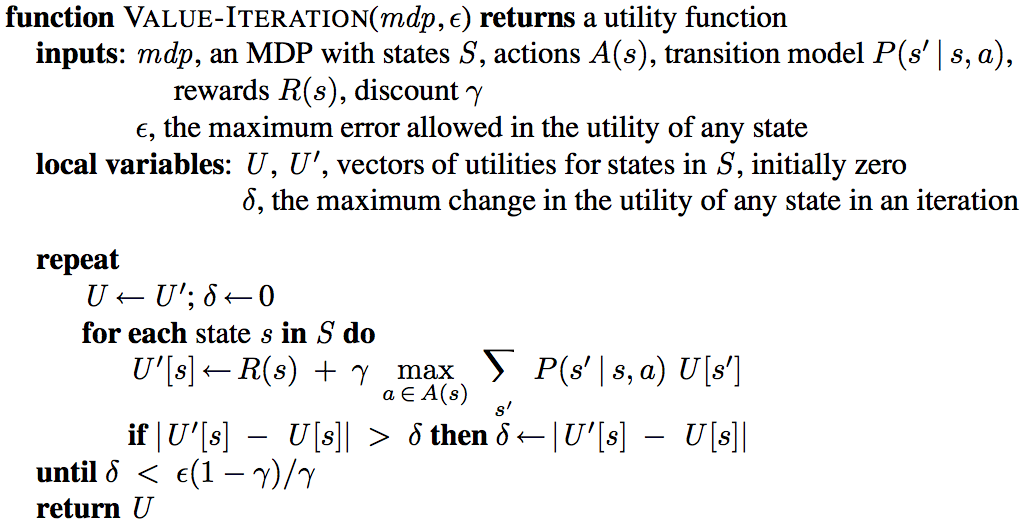
\includegraphics[width=8cm]{pics/value_iteration.png}


\subsection{Policy Iteration}
    \indent Policy Evaluation: Given a policy $\pi_i$, calculate $V_i = V^{\pi_i}$, the utility of each state if $\pi_i$ were t be executed. Do this by running Value Iteration with (or directly solving in $O(n^3)$ time the set of linear equations defined by): $V_i(s) = R(s) + \gamma \sum_{s'} P(s' | s, \pi_i(s)) V_i(s')$ \\
    \indent Policy Improvement: Calculate a new MEU policy $\pi_{i+1}$, using one-step look-ahead based on $V_i$. \\
    \indent Terminate when policy improvement yields no change in the utilities. \\
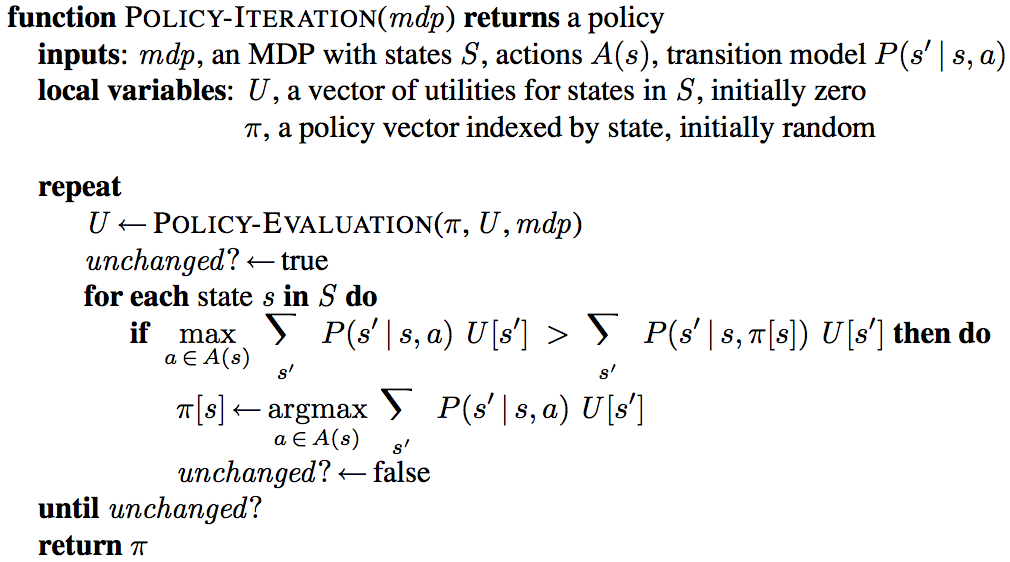
\includegraphics[width=8cm]{pics/policy_iteration.png}



\section{TD-Learning}
Off-Policy (passive) TD-Learning Update:
    $$ V^{\pi}(s) \leftarrow V^{\pi}(s) + \alpha(R(s) + \gamma V^{\pi}(s') - V^{\pi}(s)) $$
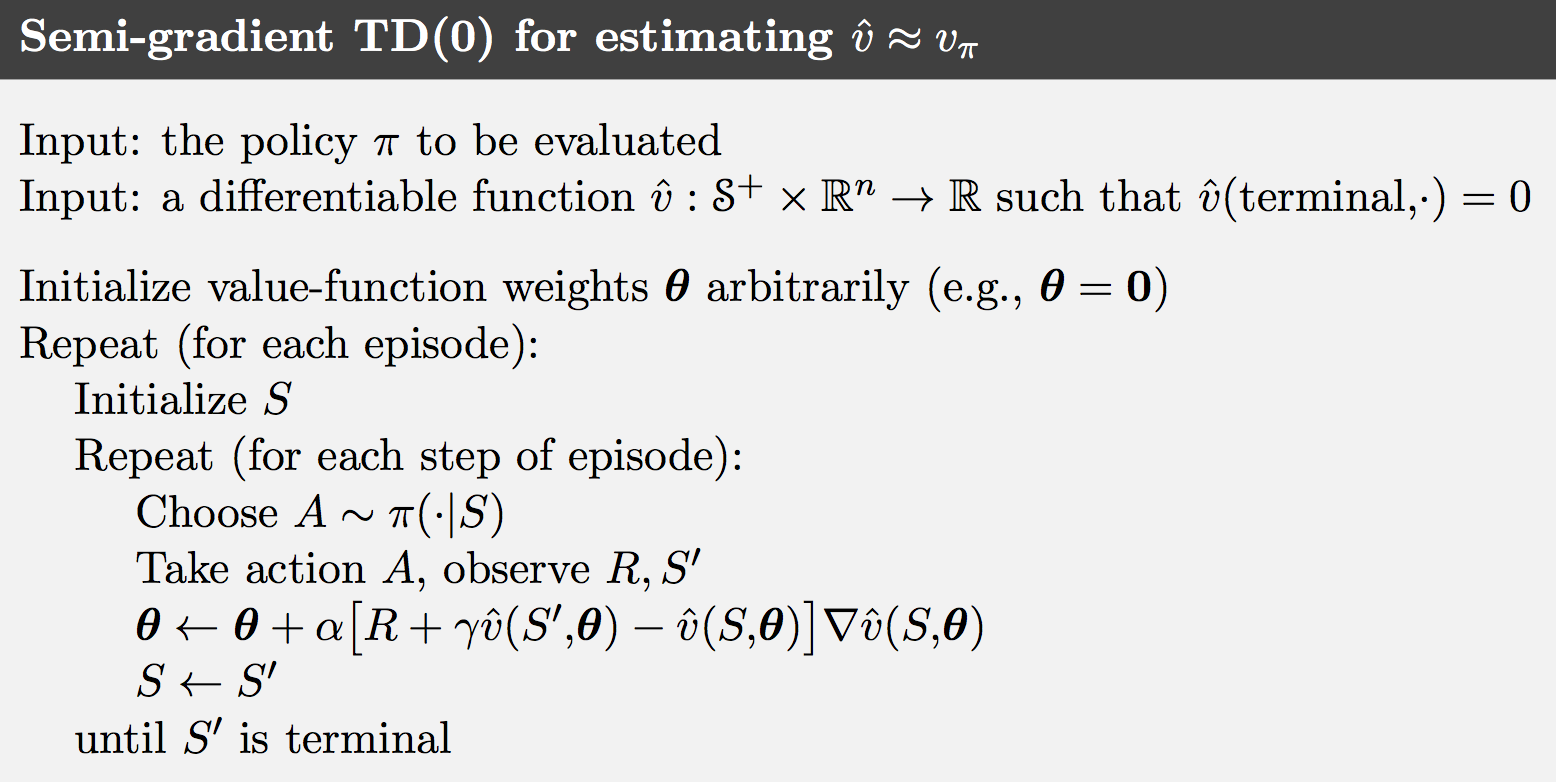
\includegraphics[width=8cm]{pics/td0_vfa.png}



\section{Monte-Carlo}
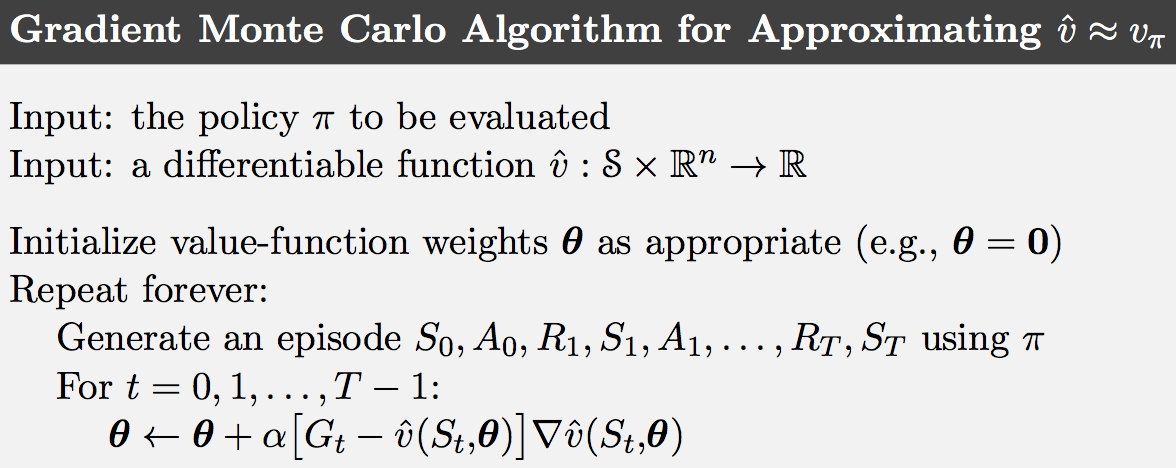
\includegraphics[width=8cm]{pics/mc_vfa.png}




\section{SARSA}
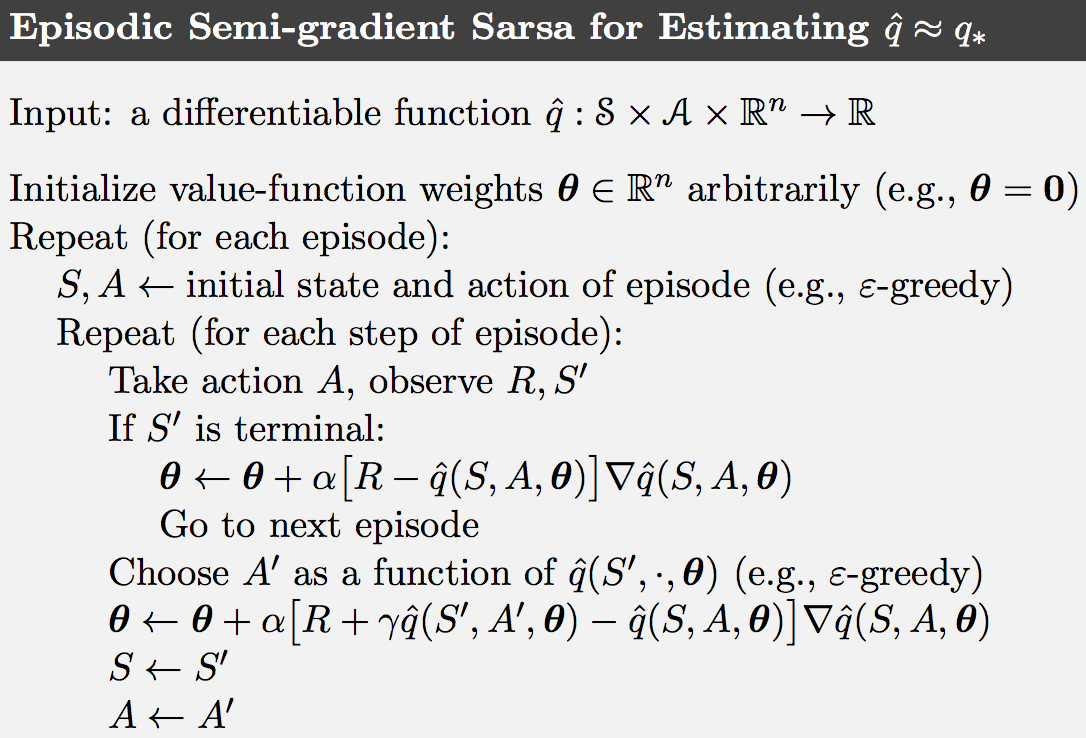
\includegraphics[width=8cm]{pics/sarsa_vfa.png}


% You can even have references
\rule{0.3\linewidth}{0.25pt}
\scriptsize
\bibliographystyle{abstract}
\bibliography{refFile}
\end{multicols}
\end{document}